\chapter{\pdsfthree{}: A Tool for \AspectOriented Modelling}
\label{chap:pdsf_rewrite}

\correctionnote{
    Is this title OK now? Worried it's too long and not sure how it renders.
    Revisit! Maybe there's a better one! Phil's original concern was that it
    makes this chapter look like there are no contributions, just a bit of
    engineering.
}

\inline{Ensure we use a consistent tense throughout}

\inline{Spell-check this chapter}

\section{Introduction}

\subsection{Chapter Outline}

The work undertaken in this thesis required an improved implementation of old
tooling. \pydysofu{} was a proof of concept which could feasibly produce
scientific models \& simulations but was implemented in a manner which was not
optimised for speed, making it a burden for large simulations. It also lacked
granularity in the application of its aspect hooks: hooks were applied to entire
classes, which forced overhead to be introduced to all attribute lookups, even
when those attributes were never intended to be used as join-points. Most
importantly, it was not compatible with Python3. \pydysofu{} manipulates Python2
objects, but Python3's objects have a changed structure which replaces their
underlying dictionaries with special classes. These enforce read-write
protections on attributes which \pydysofu{} relied on. Python2 lost official
support shortly after the work described in \cref{chap:prior_work} was
undertaken, and was not a suitable platform to build tooling on.

A new version of \pydysofu{} with support for weaving aspects in Python3 was
therefore needed; its revised implementation is named \pdsfthree{}.
\Cref{sec:pdsf3requirements} motivates in detail the development of \pdsfthree
by identifying opportunities to improve \pydysofu{}'s design.
\Cref{sec:pdsf3python3} describes approaches which were considered in the
implementation of \pdsfthree{}. The implementation of import hook weaving is
discussed in \cref{sec:import_hooks}. Other features of \pdsfthree which were
developed to improve \pydysofu{}'s maturity as a tool are given in
\cref{pdsf3_optimisations}.


\subsection{Contributions}

Implementing \pdsfthree provided an opportunity to address limitations of \aop{}
and of \pydysofu{}, thus producing a more mature tool which is appropriate for
use in research software engineering practice. In particular, \pdsfthree{}
implements a new design for the weaving of aspect hooks into prospective
join-points --- ``import hook weaving'' --- which improves the legibility of an
\aspectoriented codebase by making the application of advice more clearly
visible to a reader of that codebase. This design addresses criticism of
\aspectorientation which observes that obliviousness can make programs difficult
to read, reason about, and
maintain~\cite{Constantinides04aopconsidered,steimann06paradoxical,przybylek2010wrong,przybylek2018empirical}\footnote{These
criticisms are discussed in \cref{subsec:aop-criticisms}.}.

Import hook weaving is the most significant contribution of \pdsfthree{}. It
makes advice application more legible than other \aop{} frameworks by
restricting the ability of one area of a codebase to affect other areas, and
takes advantage of conventional Python programs' layout to place uses of \aop{}
at the top of a file. Using these design improvements, a developer can reason
about any usage of \aop{} through ``hints'' that they should be aware of \aop{}
in the codebase. As these hints are embedded in the source of a program using
\pdsfthree{}, they are provided to software engineers without need for special
tooling or static analysis.

\pdsfthree also contributes a new type of optimisation to \aop{} frameworks,
termed ``cached fuzzing''. This is an improvement to \pydysofu{}'s unique type
of join-point, ``fuzzers'' where advice is able to change the definition of the
target it is applied to. A limitation of \pydysofu is that fuzzers are applied
to their targets on every invocation of the corresponding join-point. While this allows
for dynamic fuzzer behaviour, it also forces a user of the feature to repeatedly
re-compile the target. If the result of this recompilation is the same every
time, unnecessary overhead is incurred. To alleviate this,
\pdsfthree{} offers an optimisation which caches the result of a fuzzing aspect
on its first invocation, and re-uses its cached value to avoid unnecessary
re-compilation. This is discussed in more detail in \cref{subsec:cached_fuzzing}. 

Improvements over \pydysofu{}'s original design are also addressed. For example,
\pdsfthree only weaves aspect hooks into callable values stored within modules
such as methods and functions, avoiding the overhead introduced by \pydysofu{}'s
aspect hooks when resolving non-callable attributes. \pdsfthree also offers
granular application of aspects by making use of Python's import functionality
--- if only specific functions within a module are intended to be used as
join-points, importing only those functions from the module using \pdsfthree{}'s
import hook weaving applies hooks only to those functions. This further reduces
overhead from unused join-points.

Features of other \aop{} frameworks were also missing from \pydysofu{}, which
have been added to \pdsfthree{}, such as join-points which handle raised
\lstinline{Exception}s and the ability to specify the ordering of advice
invocation. This improves the tool's maturity and brings it closer to feature
parity with other \aop{} frameworks. Exception handling aspects are discussed in
\cref{error_handling_advice}; ordering advice invocation is discussed in
\cref{aspect_priority_support}. Other optimisations are discussed throughout
\cref{pdsf3_optimisations}.


\correctionnote{
    Check that the intro to this chapter still makes sense. It's been heavily
    reworked to explain the contributions of the chapter more clearly. Is it
    clear? Does it articulate how PDSF3 improves on PyDySoFu? etcetcetc
}






\section{Requirements for Change}\label{sec:pdsf3requirements}

After developing a study using \pydysofu{}~\cite{wallis2018caise}, it became clear that an iteration on its
design was required. \pydysofu{} grew out of an undergraduate project, and accrued
technical debt as a result of being written under time constraints with little
experience. On revisiting its design and reflecting on other aspect orientation
frameworks reviewed in  
\cref{aspect_oriented_programming_litreview} and the use previously found for
\pydysofu{}~\cite{wallis2018caise,wallis2018genetic} it was clear that there were
improvements which could be made to the tool:

\begin{itemize}
    \item \pydysofu made use of techniques
      for applying aspect hooks which did not translate to the changes Python 3
      made to its object model. In particular, Python 3 changed its underlying
      object model, using a wrapper class imposing constraints on writing to
      some attributes of callable objects. This impacted the implementation of
      fuzzers, and no viable way to reimplement fuzzers using the old technique
      could be found.
    \item \pydysofu{} made no accommodations for
      efficiency. It could be seen as the ``total weaving'' described by
      \citet{dynamicAOchitchyan} as aspect hooks were implemented within the
      \lstinline{__getattribute__} method of a class, with the effect that even
      properties of the class which were not intended to be used as join-points
      were processed through \pydysofu{}'s aspect hooks. This incurred an overhead
      to their performance. In Python, the \lstinline{__getattribute__} method
      retrieves \emph{all} attributes of an object, including special built-in
      attributes and non-callable ones. Aspect hooks were therefore invoked in
      almost any scenario where a program made use of an instance of any class
      which had aspect hooks applied. As \lstinline{__getattribute__} is used by
      Python when retrieving any attribute of an object, it was not possible to
      limit the impact of \pydysofu{}'s aspect hooks to only affect potential
      join-points.
    \item \pydysofu made no accommodations for scenarios
      where fuzzing of source code was applied in a ``static'' manner. That is
      to say, where a deterministic modification to source was woven as advice,
      instead of dynamically modifying source code, the same modification would
      still be made every time the target attribute was executed, unless caching
      of results was specifically managed by the aspect applying the change. No
      optimisations were made pertaining to this, but compilation and abstract
      syntax tree editing have the potential to be \pydysofu{}'s most expensive
      operations.
    \item Unlike other aspect orientation frameworks such as
      AspectJ~\cite{aspectj_intro}, pointcuts could not be specified. Instead,
      individual join-points were be supplied as a Python object. This deviated
      from \aop{} conventions but only limited a user of \pydysofu{}: specifying a
      set of join-points was not supported by the library. Users of \pydysofu{} did
      not benefit from this lack of functionality.
\end{itemize}

As several requirements were left unfulfilled by
\pydysofu{}, a new implementation satisfying them was deemed necessary.


\section{Python3-Compatible Weaving Techniques}\label{sec:pdsf3python3}

Replacing \lstinline{__getattribute__} on the class of a targeted method was no
longer viable in Python 3. A replacement method therefore had to be found. As
discussed in \cref{subsec:prior_work_weaving}, \pydysofu{}'s technique of
replacing \lstinline{__getattribute__} allowed for hooks to be woven at runtime
into possible targets of advice. These hooks would then discover and manage the
execution of advice around each target. Because advice can be run before, after
and around a target dynamically, an alternative technique must also intercept
the calling of any target and manage advice immediately before execution. 

This section describes a search to discover alternative techniques to
dynamically weave and manage aspects which are suitable for \pdsfthree{}'s
implementation. We refer to code woven around a target which manages applied
advice as \emph{``aspect hooks''}.

The techniques of interest are specifically those which can be used to implement
\aop{} without introducing domain-specific languages (as in the case of AspectJ,
surveyed in \cref{AspectJLanguageAndTools,aspectj_intro}) or a special language
runtime (as in the case of PROSE~\cite{popovici2002PROSE} or
Nu\cite{rajan2006nu_towardsao_invocation}). \pdsfthree{} is instead implemented
in Python, requires no additional dependencies, and is used by writing native
Python code. This design is chosen for two reasons. Firstly and most
significantly, \pdsfthree would be easier to maintain in the future if it avoids
requiring a change to the Python runtime or the development and maintenance of a
domain-specific language. Changes to the language's runtime are avoided because
the Python runtime is routinely updated and changes would need to be rebased
against new Python versions. A domain-specific language is avoided because an
implementation of a new language is likely to be more complicated to implement
than a Python package: such a package is simple to implement by virtue of
Python's flexible
design~\cite{advanced_python_monkey_patching,forbiddenfruit_repo}
(described further in
\cref{subsec:pdsf3badweaving,subsec:pdsf3importhookdiscussion}). Secondly, it is
expected that the ability to use \pdsfthree{} without learning new languages or
adopting unofficial (and therefore potentially less reliable) language runtimes
may be appealing to potential users of \aop{}. This expectation could be
verified by a survey of researchers who are curious about \aspectoriented{}
modelling to investigate whether these design properties make \pdsfthree{} more
appealing than other \aop{} frameworks. This is left as future work, as there
was insufficient time remaining in this project to conduct such a survey.


\subsection{Abandoned Techniques}\label{subsec:pdsf3badweaving}

\pydysofu{} relied on ``monkey-patching'': the practice
of making on-the-fly changes to objects by ``patching''
them during program execution~\cite{advanced_python_monkey_patching}. This is
often achieved by taking advantage of language properties such as flexible
object structures~\cite{advanced_python_monkey_patching}. Common examples of
these structures are maps from string attribute / method names to the associated
underlying value, which is the model used to represent all objects in both
Python and JavaScript. Monkey-patching makes use of these structures by
replacing values such as the function object mapped to by the original
function's name in the dictionary, effectively changing its behaviour. An
example of monkey-patching in Python is given in \cref{fig:snippet-with-python-monkeypatching} This is
the method by which \pydysofu{} replaced \lstinline{_getattribute__} on a
class object.

\begin{figure}
    \centering
    \lstinputlisting[style=footnotesize_python]{40_pydysofu_rewrite/snippets/monkey_patching_example.py}
    \caption{An example of monkey-patching in Python, showing both changes to
    all instances of the \texttt{Person} class and changes to individual
    instances.}
    \label{fig:snippet-with-python-monkeypatching}
\end{figure}

Rather than relying on monkey-patching a new version of
\lstinline{__getattribute__} containing aspect hooks, the rewritten method could
be patched to the object itself at a deeper level than was available through
\pydysofu{}'s underlying mechanism. This would make use of Python's
\lstinline{ctypes} API to patch the underlying object. Similar work has been
done in the python community in a project called
ForbiddenFruit~\cite{forbiddenfruit_repo}. ForbiddenFruit uses the
\lstinline{ctypes} API to interact with the Python runtime and alter the
in-memory representation of the attributes of class objects, ``cursing'' those
objects in ForbiddenFruit's jargon.

This modification is highly dependent on the specific details of the modified
attribute. While many attributes are supported by ForbiddenFruit, cursing
\lstinline{__getattribute__} is not supported. Efforts were made to add
\lstinline{__getattribute__} cursing, but this was abandoned as the underlying
mechanism is unsafe, Python API changes could render the library unusable in
future versions of the language, and the implementation would only work with
particular implementations of Python (for \lstinline{ctypes} to exist, the
Python implementation must be written in C). Community patches existed for
cursing \lstinline{__getattribute__}, but these also could not be made to work.
There are also efficiency concerns with this technique depending on its use:
weaving advice around a function would mean monkey-patching the built-in class
of functions, which would incur an overhead from running aspect hooks on every
invocation of every function as \pydysofu{} did.

Another approach for dynamic weaving which was attempted involved making use of
existing Python functionality for interrupting method calls. As \pydysofu{}
wrapped method calls dynamically, what was required was to add program logic to
the beginning and end of the execution of a method. Python has features
providing this functionality which were designed for the implementation of
debuggers, profilers, and similar development tools. The built-in function
\lstinline{settrace} allows a developer to specify a function which is invoked
on certain events in Python's runtime. The intended use case for
\lstinline{settrace} is to track function invocations and exceptions being
raised --- however, the existence of a function invocation event suggested that
\pdsfthree{} could dynamically apply aspects by using this functionality.

Making use of \lstinline{settrace} also has issues. Most significantly,
\lstinline{settrace} catches myriad events in the Python interpreter which
\pdsfthree{} is unconcerned with, which incurs significant overhead. In
addition, only one callback can be set using \lstinline{settrace}, meaning that
any programmer would have to choose between using a debugger and using
\pdsfthree{}. This was deemed untenable: debuggers are an important development
tool and a weaving approach which prevents their use was not realistically
useful. However, future Python versions may change their design of
\lstinline{settrace} in a way which makes this weaving approach feasible. If
future versions of the language allow for multiple trace handlers, this could
provide a promising alternative approach to the implementation of future dynamic
aspect orientation frameworks.


\subsection{Import Hooks}\label{subsec:pdsf3importhookdiscussion}

A final available technique is to continue to monkey-patch hooks to discover and
weave aspects, via an alternative method which does not make use of
\lstinline{__getattribute__}. This approach would change the use of \pdsfthree{}
to make a compromise between performance and obliviousness of aspect
application: when importing a module targeted for aspect weaving, potential
target methods are monkey-patched with a wrapper method with a reference to the
original --- necessary to run the targeted method --- and hooks to detect and
run dynamically supplied advice.

Many behaviours of objects in Python are defined through their ``magic
methods'' (as mentioned in \cref{first_reference_to_magic_methods}). Magic method
identifiers begin and end with two underscore (\lstinline{_}) characters and
have special meanings within Python. The Python language documentation specifies
sets of magic methods and their required function signatures which are used
internally to implement functionality~\cite{py3docs}. For example, any object
with the method \lstinline{__eq__} defined can be compared against using the
\lstinline{==} operator, and the \lstinline{__eq__} magic method is run to
determine the outcome of the operator. Magic methods are also used for more
complex Python functionality: they determine whether they satisfy the conditions
of some Python's categories of objects. For example, anything which defines
\lstinline{__len__} and \lstinline{__getitem__} is treated as an immutable
container, and adding \lstinline{__setitem__} and \lstinline{__delitem__} makes
that container mutable. Any class defining \lstinline{__call__} is treated as a
callable object akin to a function: when the object is called, the
\lstinline{__call__} magic method is executed. More can be found in Python's
documentation~\cite{py3docs}, although more focused guides exist in the Python
community~\cite{magicmethodguide}.

Magic methods make Python ideal for implementing import-based weaving of aspect
hooks, particularly dynamically, as they can be overridden. Python's
functionality for importing modules is managed by
\lstinline{builtins.__import__}, which receives module names as strings and
handles package resolution; by monkey-patching the import system, modules can be
modified during the process of importing. As this technique allows for control
over where aspect hooks are applied, \pdsfthree can target only function and method
objects to apply aspect hooks to, avoiding the overhead \pydysofu
introduced when applying hooks to all attribute lookups including non-callables,
such as variables or \lstinline{Class} objects. \footnote{A successor to
\pdsfthree{} could hypothetically be extended to apply advice to attributes instead
of functions or methods, as was possible with the previous version's weaving
technique using \lstinline{__getattribute__}. However, it is unclear how this
could be implemented as the new weaving technique relies on target
\emph{invocation}, meaning only callables are viable targets. The additional
research overhead of devising a technique to apply advice to aspects when their
values are resolved was deemed too great to justify the investment given this
functionality was not required for the work at hand. Python's
\lstinline{@property} decorator turns methods of classes into properties of
those classes; as this would allow properties to be represented internally as
methods, and so as possible join-points with \pdsfthree{}, an
investigation into this decorator could yield a viable approach. This is
suggested as potential future work on the \pdsfthree{}.}

Monkey-patching \lstinline{builtins.__import__} is as simple as replacing the
\lstinline{__import__} function object with a new one, which changes the
behaviour of Python's \lstinline{import} keyword. Because all Python
functionality relies on magic methods implicitly, its behaviour can be altered
in this way. However, the intent is not necessarily to manipulate \emph{all}
modules, but a subset of imports specified by a modeller as suitable for
manipulation. If all invocations of \lstinline{import} wove hooks into modules,
including those made while \emph{already} in the process of importing packages,
an unnecessary overhead would be introduced when invoking any module and another
overhead would be incurred executing the aspect hooks on any callable imported
by any module. For this reason it is important to have a mechanism to enable and
disable the weaving of aspect hooks for a given \lstinline{import} statement,
requiring a mechanism to enable and disable \pdsfthree{}'s modified import logic.

Monkey-patching \lstinline{builtins.__import__} can be achieved through another
use of magic methods in a manner which also makes clear to a modeller exactly
where aspect hooks are being applied: making use of Python's \lstinline{with}
keyword, which uses the \lstinline{__enter__} and \lstinline{__exit__} magic
methods to define a block of code where an arbitrary resource such as a file,
mutex, or network connection is safely managed. This behaviour is
exapted\footnote{\citet{exaptation_origin} coined the term ``exaptation'' to
refer to a trait of a species which evolved in response to one need, but were
later co-opted to satisfy another.} by \pdsfthree{} to manage the behaviour of the
import keyword, creating a block of code where aspect hooks can be injected into
modules as they are imported. As these are a core component of \pdsfthree{}'s weaving
implementation, a deeper explanation of Python's \lstinline{with} keyword
follows in \cref{pdsf3implementingimporthooks} following a technical discussion
of the new weaving process which gives context to its design and implementation.



\section{\pdsfthree{}'s Import Hook Weaving}\label{sec:import_hooks}

\Cref{sec:pdsf3python3} surveyed mechanisms to implement dynamic aspect hook
weaving which did not rely on a domain-specific language or changes to language
runtimes. Some potential mechanisms were described in
\cref{subsec:pdsf3badweaving} which were ultimately deemed infeasible to adopt
for performance reasons, maintenance burden, and the difficulty of using those
mechanisms with other developer tools. In
\cref{subsec:pdsf3importhookdiscussion} it was determined that weaving aspect
hooks as modules are imported was viable. The implementation of import hook
weaving and its use in implementing an \aop{} framework is discussed in this
section.


\subsection{High-Level Description of Weaving Process}\label{subsec:pdsf3_weaving_process}

Weaving in \pdsfthree{}~\cite{pdsf_source_in_analysis_repo}
takes place via monkey-patching of aspect hooks, described in detail in
\cref{pdsf3implementingimporthooks}. Aspect hooks replace executable targets
within a module at the moment the module is imported. When the target is
invoked, the wrapping aspect hook is executed in lieu of the original target
object. The wrapping aspect contains the target function within its closure,
allowing it to execute the original target; however, it was also created by the
\lstinline{AspectHooks} class, and so has reference to aspects registered
against it. 

The high-level process of using \aop{} with \pdsfthree{}'s import hook weaving is as
follows (visualised in \cref{fig:high-level-import-hook-weaving-steps}):

\begin{enumerate}\label{urgency_mentioned_in_passing}
    \item A module which will be the target of later aspect application is
    imported using \lstinline{AspectHooks}. This replaces callable objects in
    the module with wrappers of those objects which contain aspect hooks. The
    process involved in this step is explained in detail when discussing
    implementation details in \cref{pdsf3implementingimporthooks}. A simple
    example is shown in \cref{fig:simple_example_of_aspect_weaving} on lines
    \texttt{1}--\texttt{3}. 
    \item An aspect is registered against \lstinline{AspectHooks}. A simple
    example is shown in \cref{fig:simple_example_of_aspect_weaving} on line
    \texttt{8}. More detailed examples are given in
    \cref{examples_of_using_pdsf} following an explanation of their
    implementation. A pointcut is specified by providing a regular expression
    matching the names of intended join-points as the first argument to an
    aspect registering method of \lstinline{AspectHooks}; their second arguments
    are the advice to apply. Available aspect registration methods are described
    in \cref{aspect_registration_methods}. Note that\ldots{}:
    \begin{itemize}
        \item Invoking the above aspect hook registration methods compiles and
        caches the regular expression provided, improving the efficiency of
        using the regular expression to identify join-points in later target
        invocations.
        \item Each aspect registration method returns a callback which de-registers
        the registered aspect. This facilitates the dynamic application of
        aspects.
    \end{itemize}
    \item  An invocation of a function or method within that module triggers
    \pdsfthree{}'s aspect hooks, which dynamically discover aspects registered
    against themselves using aspects' pointcuts. These pointcuts are described
    by the regular expressions they were registered with. Any aspects which are
    discovered are executed appropriately, as described later in
    \cref{building_aspect_Hook_wrappers}.
\end{enumerate}

\begin{figure}
  \centering
  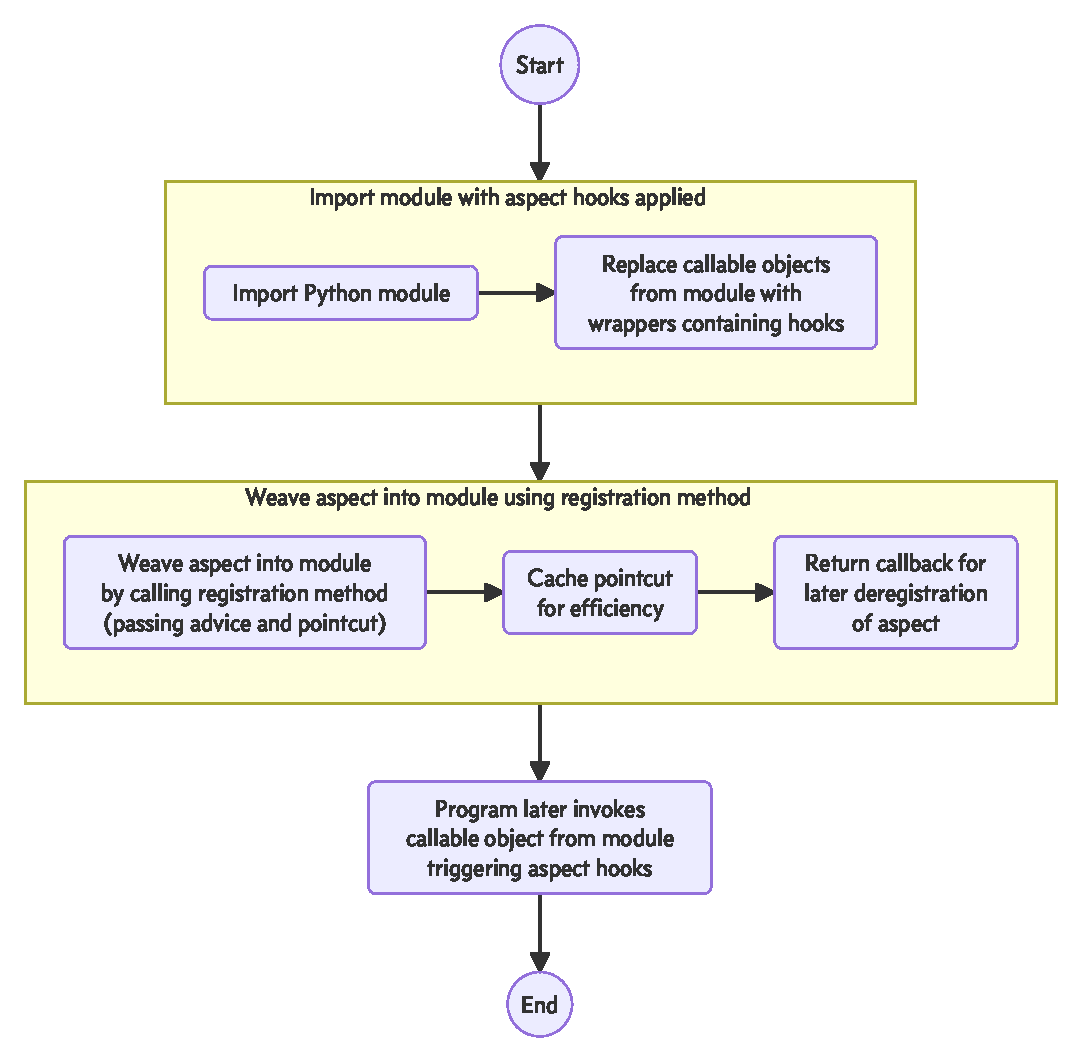
\includegraphics[width=0.8\columnwidth]{40_pydysofu_rewrite/diagrams/aspect-hook-weaving-high-level.pdf}
  \caption{Flowchart showing the high-level process of using \aop{} through
  \pdsfthree{}'s import hook weaving, as described in
  \cref{subsec:pdsf3_weaving_process}. This involves weaving aspect hooks into a
  module, applying advice to point-cuts, and invoking a join-point within the
  specified point-cut to trigger the advice.}
  \label{fig:high-level-import-hook-weaving-steps}
\end{figure}


\begin{figure}
    \begin{lstlisting}[style=footnotesize_python]
from pdsf import AspectHooks
with AspectHooks():
    import some_module
    
def prelude_advice(target, *args, **kwargs):
    print(f"Invoking {target.__name__}.")

AspectHooks.add_prelude("*some_func*", prelude_advice)
    \end{lstlisting}
    \caption{A simple example of aspect weaving, showing a prelude aspect definition, the injection of aspect hooks into a module, and the registration of advice against those aspect hooks, with pointcuts defined as regular expressions. Specific details of each step are given in later subsections as appropriate.}
    \label{fig:simple_example_of_aspect_weaving}
\end{figure}

\begin{table}
    \centering
    \begin{tabular}{@{}lp{0.55\textwidth}@{}}
        \toprule
        \emph{Method Name} & \emph{Description}\\
        \midrule
        \lstinline[]$add_prelude(rule, aspect)$ &
            Registers advice to be run before a target is invoked\\
        \rule{0pt}{2em}\lstinline[]$add_encore(rule, aspect)$ &
            Registers advice to be run after a target is invoked\\
        \rule{0pt}{2em}\lstinline[]$add_around(rule, aspect)$ &
            Registers advice to wrap an aspect invocation, effectively providing
            the functionality of \lstinline[]$prelude$ and \lstinline[]$encore$
            advice with a single aspect\\
        \rule{0pt}{2em}\lstinline[]$add_error_handler(rule, aspect)$ &
            Registers advice to catch and process exceptions raised by a join-point\\
        \rule{0pt}{2em}\lstinline[]$add_fuzzer(rule, aspect)$ &
            Registers advice to modify a target before it is invoked,
            effectively providing aspect application within a join-point, and
            permits arbitrary modifications of the target at the level of the
            abstract syntax tree.\\
        \bottomrule
    \end{tabular}
    \caption{Methods of the \lstinline{AspectHooks} class which are used to
    register different types of aspect to be dynamically woven. All methods take
    a string-represented regular expression describing the aspect's pointcut,
    and a callable object as the aspect to apply to that pointcut. The aspect
    should have the appropriate function signature for the type of advice being
    woven, as described in \cref{fig:types_of_advice}. Each method also accepts an
    optional \lstinline{urgency} integer parameter, enabling optional additional
    features of \pdsfthree{}. This optimisation is explained after implementation
    details are discussed; more details are given in
    \cref{aspect_priority_support}.}
    \label{aspect_registration_methods}
\end{table}

\pdsfthree{} advice is implemented as callable objects (usually functions). Different
types of advice have different function signatures; the arguments expected by
each type of advice are given in \cref{fig:types_of_advice}. In the arguments for
each type of advice listed in the table: \lstinline{target} is the target an
aspect is applied to; \lstinline{target_return_val} is the value returned by a
target after it was run; \lstinline{next_around} is what an
\lstinline{around}-style advice runs when it has finished its pre-target
component, and intends to run the target itself;
\lstinline{ast_steps} is a list of AST objects representing the
definition of the target a fuzzing aspect is applied to; and
\lstinline{*args,}~\lstinline{**kwargs} is a Python idiom collecting a
function's positional and keyword arguments respectively which were passed into
the function when it was invoked but was not specified within its signature.
These are used in the signatures of advice to collect arguments passed to a
target, and can be inspected by any aspect, and passed into the target if the
aspect invokes it.

\begin{table}
    \centering
    \begin{tabular}{@{}lll@{}}
        \toprule
        \begin{tabular}{@{}l@{}}\emph{\pdsfthree{}}\\\emph{Type of Advice}\end{tabular} &
        \begin{tabular}{@{}l@{}}\emph{Common Name}\\\emph{In Literature}\end{tabular} &
        \begin{tabular}{@{}l@{}}\emph{Arguments Accepted 
        by}\\\emph{Aspect Implemented in \pdsfthree{}}\end{tabular} \\
        \midrule
        \lstinline[]$prelude$ & ``before''-style & \lstinline[]$target, *args, **kwargs$\\
        \rule{0pt}{2em}\lstinline[]$encore$ & ``after''-style & \lstinline[]$target, target_return_val, *args, **kwargs$\\
        \rule{0pt}{2em}\lstinline[]$around$ & ``around''-style & \lstinline[]$next_around, target, *args, **kwargs$\\
        \rule{0pt}{2em}\lstinline[]$error\_handler$ & error handler & \lstinline[]$target, handled_exception, *args, **kwargs$\\
        \rule{0pt}{2em}\lstinline[]$fuzzer$ & ``within''-style & \lstinline[]$ast_steps, target, *args, **kwargs$\\
        \bottomrule
    \end{tabular}
    \caption{Different types of advice supported by \pdsfthree{} and the arguments
    they expect}
    \label{fig:types_of_advice}
\end{table}


Most types of advice are named using the metaphor of a play, drawing on early
\theatreag{} work as described in \cref{subsec:prior_work_theatre}:
\lstinline{prelude}, \lstinline{encore}, and \lstinline{around} advice runs
before, after, and before \& after the target respectively. Also following the
naming scheme used by \pydysofu{} are \lstinline{fuzzer}
aspects, which operate within their targets. The common names of these types of
aspects in other literature, also shown in \cref{fig:types_of_advice}, make
clear how their invocation relates to the invocation of the target they are
applied to. The term ``within'' is introduced to conform to the positional
naming convention used by other tools (``before'', ``after'', and ``around''). A
type of advice not present in \pydysofu{} is
\lstinline{error_handler} advice, which catches and attempts to handle
exceptions raised by a target.

\begin{figure}
    \begin{lstlisting}[style=footnotesize_python]
@classmethod
def add_around(cls, rule, advice, urgency=0):
    rule_tuple = (re.compile(rule), advice, urgency)
    AspectHooks.around_rules.append(rule_tuple)
    return lambda : AspectHooks.around_rules.remove(rule_tuple)
    \end{lstlisting}
    \caption{Implementation of the \lstinline{add_around} method of the
    \lstinline{AspectHooks} class, used to associate some advice ($3^{rd}$
    argument) to a pointcut, specified by a regular expression ($2^{nd}$
    argument). The \lstinline{urgency} argument is related to an optimisation
    in the tool, and is described in \cref{aspect_priority_support}. Its first
    argument is an ancillary implementation detail related to the
    \lstinline{classmethod} decorator.}
    \label{fig:add_around_impl}
\end{figure}


\lstinline{AspectHooks} methods which register methods are all implemented
similarly. The implementation of the \lstinline{add_around} method is given in
\cref{fig:add_around_impl}. It requires two arguments: advice to apply, and a
string-formatted regular expression describing the pointcut which this advice
should be applied to. Line \texttt{3} constructs an aspect from the advice and
pointcut passed as arguments, and line \texttt{4} adds this aspect to a list of
around aspects, which is searched as required when potential join-points are
invoked. This is described in further detail in
\cref{injecting_aspect_hooks_when_importing}. It returns a lambda which
deregisters the aspect. Detailed examples using these methods to register
aspects are given in \cref{examples_of_using_pdsf}.


\subsection{Controlling Import Behaviour using Python's \lstinline{with} Blocks}
\label{pdsf3implementingimporthooks}

To inject aspect hooks into modules when importing them, \pdsfthree{} must
modify \lstinline{builtins.__import__} \emph{only} when modules containing
potential join-points are imported. A developer might import many modules
which do not require aspect hooks to be introduced: introducing hooks to all
modules would incur some overhead from the hooks themselves when invoking any
callable in any module. To enable this, \pdsfthree{} uses Python's
\lstinline{with} keyword, as demonstrated in
\cref{fig:simple_aspect_hook_weaving_example}. The use of \lstinline{with AspectHooks()}
in \cref{fig:simple_aspect_hook_weaving_example} monkey-patches
all potential targets of advice in the \lstinline{mymodule} package to inject
aspect hooks into them.

\begin{figure}
    \centering
    \begin{lstlisting}[style=footnotesize_python]
with AspectHooks():
    import mymodule
    \end{lstlisting}
    \caption{Example of importing a module named \lstinline{mymodule} using
    \pdsfthree{}'s import hook design. This code snippet weaves aspect hooks into all
    functions and non-builtin class methods within the \lstinline{mymodule}
    module object, and this modified module is added only to the local namespace
    of the importing stack.}
    \label{fig:simple_aspect_hook_weaving_example}
\end{figure}

\begin{figure}
    \centering
    \begin{lstlisting}[style=footnotesize_python]
import sys
import copy

class AspectHooks:
    def __enter__(self, *args, **kwargs):
        self.old_import = __import__
        self.old_modules = copy.copy(sys.modules)
        self.imported = set()
        import builtins
        builtins.__import__ = self.__import__

    def __import__(self, *args, **kwargs):
        if args[0] in sys.modules:
            del sys.modules[args[0]]
        mod = self.old_import(*args, **kwargs)
        self.imported.update([args[0]])
        
        def apply_hooks(target_object):
            # ...implementation snipped

        apply_hooks(mod)
        return mod

    def __exit__(self, *args, **kwargs):
        builtins.__import__ = self.old_import
        for i in self.imported:
            if i in self.old_modules:
                sys.modules[i] = self.old_modules[i]
            else:
                del sys.modules[i]
        self.imported = set()
    \end{lstlisting}
    \caption{\pdsfthree{} implementation of the magic methods used by a Python
    \lstinline{with} block to alter import behaviour.}
    \label{fig:aspecthooksmagicmethodswith}
\end{figure}

\correctionnote{Consider adding a pseudocode example here for explaining how with blocks get used in practice.}

The behaviour of Python's \lstinline{with} keyword can be explained through the magic
methods which enable it: when entering a \lstinline{with} block, the
\lstinline{__enter__} method on the object
following the \lstinline{with} keyword is invoked. When exiting the block, its
\lstinline{__exit__} method is invoked. It is only valid to enter a
\lstinline{with} block by using an object with both magic methods defined. The
\lstinline{AspectHooks} class uses these methods to override Python's import
functionality when entering the block by replacing
\lstinline{builtins.__import__}, and reverts to the original functionality when
exiting the block. The implementation of these methods is shown in
\cref{fig:aspecthooksmagicmethodswith}.

When entering the block, the original import function is stored and replaced by
a method of the \lstinline{AspectHooks} instance. This is shown on lines
\texttt{6}, \texttt{9} and \texttt{10} of
\cref{fig:aspecthooksmagicmethodswith}. The original function is used to
import modules on line \texttt{15}, but the module it returns is altered by
\pdsfthree{} by injecting aspect hooks on line \texttt{21}. The mechanism for
applying these hooks is explained in \cref{injecting_aspect_hooks_when_importing}.
The original implementation of \lstinline{builtins.__import__} is restored on
line \texttt{25}, ensuring that import behaviour is only altered within the
\lstinline{with} block.


\subsection{Locally Injecting Aspect Hooks}
\label{local_aspect_hook_effects}

Before discussing how aspect hooks are injected into a module object, an
additional piece of functionality shown in
\cref{fig:aspecthooksmagicmethodswith} must be explained. \pdsfthree{} ensures
that modules only have aspect hooks where the module is imported with
\lstinline{AspectHooks}, rather than every time the module is imported. An
example of this behaviour is illustrated in
\cref{fig:isolated_aspect_hook_weaving_illustration_reproduced}.


\begin{figure}
    \centering
    \lstinputlisting[style=footnotesize_python,captionpos=t,title={\raggedright{}\footnotesize{}\texttt{main.py}}]{40_pydysofu_rewrite/snippets/isolated_hook_weaving/main.py}
    \lstinputlisting[style=footnotesize_python,captionpos=t,title={\raggedright{}\footnotesize{}\texttt{joinpointModule.py}}]{40_pydysofu_rewrite/snippets/isolated_hook_weaving/joinpointModule.py}
    \lstinputlisting[style=footnotesize_python,captionpos=t,title={\raggedright{}\footnotesize{}\texttt{aspects.py}}]{40_pydysofu_rewrite/snippets/isolated_hook_weaving/aspects.py}
    \lstinputlisting[style=footnotesize_python,captionpos=t,title={\raggedright{}\footnotesize{}\texttt{moduleA.py}}]{40_pydysofu_rewrite/snippets/isolated_hook_weaving/moduleA.py}
    \lstinputlisting[style=footnotesize_python,captionpos=t,title={\raggedright{}\footnotesize{}\texttt{moduleB.py}}]{40_pydysofu_rewrite/snippets/isolated_hook_weaving/moduleB.py}
    \caption{Example Python project with multiple modules, which demonstrate how
    \pdsfthree isolates \aspectoriented behaviour to affect only modules which
    import join-points with \lstinline{AspectHooks}. Here, \lstinline{moduleA}
    weaves an aspect into \lstinline{joinpointModule}, but \lstinline{moduleB}
    does not observe any \aspectoriented behaviour because it did not import
    \lstinline{joinpointModule} with \lstinline{AspectHooks}.}
    \label{fig:isolated_aspect_hook_weaving_illustration_reproduced}
\end{figure}


Additional work is necessary for this behaviour, because Python's
default import logic caches modules and uses the cached module objects when
importing a second time~\cite{python_import_cache_definition}. This cache is
stored in \lstinline{sys.modules}. If hooks are applied to a module within this
cache, \emph{every} part of a program which imports that module will include
hooks, as every time the module is imported the same object is returned. This
would lead to previous imports of a module which is imported using
\lstinline{AspectHooks} to have altered behaviour, even though aspect hooks were
injected in an unrelated part of a program. This is similar to the behaviour of
other \aop{} approaches, such as AspectJ~\cite{AspectJLanguageAndTools}: aspects
can be applied to a pointcut anywhere in a program. However, this makes code
difficult to reason about~\cite{steimann06paradoxical,przybylek2010wrong}.
\pdsfthree{} improves on the legibility of \aspectoriented programs by
\emph{only injecting hooks where \pdsfthree{} has been invoked}, affecting the
program locally rather than globally. To achieve this, Python's cache of
previously imported modules must be managed.

Management of this cache is explained using the implementation shown in
\cref{fig:aspecthooksmagicmethodswith}.

When entering a \lstinline{with} block using an instance of the
\lstinline{AspectHooks} class, the instance's \lstinline{__enter__} method is
called. This method stores a copy of the modules imported when entering the
block on line \texttt{7} of \cref{fig:aspecthooksmagicmethodswith}. This is used
later to ensure that the cache contains the versions of any imported module
which do not contain aspect hooks when exiting the \lstinline{with} block. On
line \texttt{8}, a set of all modules imported while inside the block is
initialised. This is used to identify which modules' states must be reset when
leaving the block.

Before leaving the block, \pdsfthree{} modifies Python's import logic to inject
aspect hooks. The \lstinline{if} statement on \texttt{13} of
\cref{fig:aspecthooksmagicmethodswith} checks whether the module being imported
already exists in the cache. If it does, it is removed from the cache, so that
when Python's usual import function is later invoked it re-imports the module
rather than relying on the cache. The usual import function is invoked on line
\texttt{15}. This returns a new module object, and also adds this module object
to the cache. The rest of this function injects aspect hooks into the module.

When exiting the \lstinline{with} block, the cache should be returned to its
expected state. Any modules which were altered by \pdsfthree{} exist in the cache of
imported modules, and should be replaced with their expected values: if they
previously existed in the cache, the previous object without aspect hooks should
replace the one currently residing in the cache. If it did not previously exist,
the object should be removed from the cache entirely, so that later import
statements re-import the module and construct a new module object which lacks
aspect hooks. This check is performed by the \lstinline{for} loop on line
\texttt{26} of \cref{fig:aspecthooksmagicmethodswith}. Previously existing
modules replace those constructed by \pdsfthree{} on line \texttt{28}, and new
entries in the cache are deleted on line \texttt{30}.

Following these steps, the state of Python's module cache is managed to avoid
modules imported elsewhere without \pdsfthree{} from containing aspect hooks.

\subsection{Injecting Aspect Hooks Into Modules}
\label{injecting_aspect_hooks_when_importing}

\Cref{fig:apply_hooks_to_module} shows the implementation of the
\lstinline{apply_hooks} function, referenced on line \texttt{21} of
\cref{fig:aspecthooksmagicmethodswith}. This function searches an
object for functions and methods which are possible targets of advice, injecting
aspect hooks into each one. Any classes contained within the object are searched
recursively.

\begin{figure}
    \centering
    \begin{lstlisting}[style=footnotesize_python]
from inspect import isfunction, ismethod, isclass
from functools import filter

def build_wrapper(callable_object):
    # ...implementation snipped.
    # Builds a wrapper around `callable_object` containing aspect hooks
    # and returns the wrapped object.

def apply_hooks(target_object):
    nonprivate = lambda p: isinstance(p, str) and len(p) > 1 and p[:2] != "__"\\
    for item_name in filter(nonprivate, dir(target_object)):
        item = getattr(target_object, item_name)

        from_mod = getattr(item, "__module__", None) == mod.__name__
        if from_mod or AspectHooks.deep_apply:
            if isfunction(item) or ismethod(item):
                setattr(target_object, item_name, build_wrapper(item))
            elif isclass(item):
                apply_hooks(item)
    \end{lstlisting}
    \caption{The implementation of the \lstinline{apply_hooks} function used on
    line \texttt{21} of \cref{fig:aspecthooksmagicmethodswith}, which injects
    aspect hooks into any function or method within a module object or the
    classes it contains. Edited slightly for legibility.}
    \label{fig:apply_hooks_to_module}
\end{figure}

Line \texttt{10} of \cref{fig:apply_hooks_to_module} defines the condition used
to filter attributes of \lstinline{target_object}, which is a module object when
\lstinline{apply_hooks} is first called, but a class object on recursive
invocations, as explained later. The condition on which an attribute of an
object is checked as a possible join point is that it is a string with at least
two characters and where the first two characters are not underscore (\_)
characters. This ensures that protected attributes, which are idiomatically
prepended with two underscore (\_) characters, are not accidentally used as
targets for advice. These methods typically have special meanings within Python
and could introduce unexpected side-effects and significant performance
overheads if their behaviours are changed by advice. This condition is used to
filter out attributes of \lstinline{target_object} which would be unsuitable
join-points on line \texttt{11}. Attributes which are suitable join-points are
retrieved from the object on line \texttt{12}.

Line \texttt{14} of \cref{fig:apply_hooks_to_module} checks whether the
prospective join point belongs to the same module as the one being imported. The
variable \lstinline{mod} is defined elsewhere, as it refers to the module being
imported: the code shown in \cref{fig:apply_hooks_to_module} is the snippet
truncated from line \texttt{19} of \cref{fig:aspecthooksmagicmethodswith}. This
functionality is related to the deep hook weaving optimisation explained later
in \cref{deep_hook_weaving} --- lines \texttt{14} and \texttt{15} will be
explained as needed when discussing this optimisation.

Lines \texttt{16}--\texttt{19} of \cref{fig:apply_hooks_to_module} inject aspect
hooks into \lstinline{target_object} if appropriate. If the object is a function
or method, it is replaced within the imported module. Its replacement is a
new function or method built by the \lstinline{build_wrapper} function, which wraps
\lstinline{target_object} with aspect hooks. However, if
\lstinline{target_object} is a class, it is not callable (and so cannot be a
join-point) but may \emph{contain} functions or methods which would be valid
join-points. To inject aspect hooks into these, \lstinline{apply_hooks} is
called recursively on the class object.

Calls to \lstinline{apply_hooks} modify the objects passed as arguments
directly. As a result, they need not return any value. All functions
and methods which are suitable join-points have been replaced with wrappers
implementing aspect hooks at this point, and so the work required to be done on
the imported module object is done, and aspect hooks are injected into it at all
appropriate points.


\subsection{Building Wrappers With Aspect Hooks}
\label{building_aspect_Hook_wrappers}

\begin{figure}
    \centering
    \lstinputlisting[style=scriptsize_python,linewidth=1.05\columnwidth]{40_pydysofu_rewrite/snippets/build_wrapper_impl.py}
    \caption{The implementation of \lstinline{build_wrapper}, which takes a
    function or method as an argument and returns that object wrapped with logic
    implementing aspect hooks. Edited slightly for legibility.}
    \label{fig:build_wrapper_impl}
\end{figure}

\begin{figure}
    \centering
    \lstinputlisting[style=footnotesize_pseudocode,mathescape]{40_pydysofu_rewrite/snippets/build_wrapper.pseudocode}
    \caption{Pseudocode explaining how \lstinline{build_wrapper} works. The
    implementation is given in \cref{fig:build_wrapper_impl}.}
    \label{fig:build_wrapper_pseudocode}
\end{figure}


\Cref{fig:build_wrapper_impl} shows the implementation of the
\lstinline{build_wrapper} function, which takes a function or method as an
argument and returns that argument wrapped inside a function which invokes
advice. The \lstinline{build_wrapper} function is used by the
\lstinline{apply_hooks} function as shown in \cref{fig:apply_hooks_to_module} to
inject aspect hooks into functions and methods modules and classes they contain.

This code snippet is large, but there are six areas of particular importance to
the discussion of \pdsfthree{}'s implementation. Lines \texttt{2}--\texttt{13}
construct some foundations used by other parts of the implementation. Lines
\texttt{17}--\texttt{41} implement ``within''-style aspects (fuzzers). Prelude
advice is handled by line \texttt{44}. Lines
\texttt{50}--\texttt{57} invoke ``around''-style aspects, and also invoke the target
of any advice applied. Lines
\texttt{60}--\texttt{64} invoke ``after''-style aspects, and handle the return
value of the target. Finally, lines \texttt{66}--\texttt{72} handle exceptions
raised by the target or any advice applied, using exception handling advice.
These will be explained individually.

\subsubsection{Initial Setup}
Lines \texttt{2}--\texttt{13} of \cref{fig:build_wrapper_impl} contain setup for
later parts of the \lstinline{build_wrapper} function.

A copy of the original code object of the target being invoked is stored on line
\texttt{2}. This is required to restore its state if fuzzers are applied. This
state is restored by calling a function, \lstinline{reset_code_to_previous},
implemented on lines \texttt{9}--\texttt{13}. An exception to be raised if an
error is encountered during fuzzing is implemented on lines
\texttt{3}--\texttt{4}. The aspects which apply to the target being invoked are
retrieved by a call to another function, \lstinline{get_rules}, on line
\texttt{8}. \revnote{The name of get\_rules feels like a mistake I never
corrected. If there's time before submission, fix this. If not, it really
doesn't matter.}

\subsubsection{Fuzzers}

Lines \texttt{17}--\texttt{41} of \cref{fig:build_wrapper_impl} implement
\pdsfthree{}'s ``within''-style aspects, or fuzzers. A pseudocode representation
of the process is given in \cref{fig:fuzzer_impl_pseudocode}.
Lines \texttt{19}--\texttt{22} implement a static fuzzing optimisation, which is
discussed later in \cref{static_weaving}. Their explanation is omitted here, and
included in \cref{static_weaving} instead.

\begin{figure}
    \centering
    \lstinputlisting[style=footnotesize_pseudocode,mathescape]{40_pydysofu_rewrite/snippets/fuzzer.pseudocode}
    \caption{A pseudocode representation of the process used to apply fuzzers to
    the targets of advice. This is a simplification of the implementation given
    in \cref{fig:build_wrapper_impl}.}
    \label{fig:fuzzer_impl_pseudocode}
\end{figure}

The target being invoked is fuzzed on lines \texttt{24}--\texttt{36}. The
original source code of the target is retrieved using Python's built-in
\lstinline{inspect} library, and indentation is removed to avoid errors when
recompiling. An AST is constructed from this source code, and the part of that
AST representing the body of the function implementation is stored in the
\lstinline{funcbody_steps} variable. Lines \texttt{28}--\texttt{30} contain a
\lstinline{for} loop which calls every fuzzer applied to the target. Each fuzzer
takes an AST as an argument and returns a replacement AST with any
transformations it applies. By the end of this \lstinline{for} loop, the AST
stored in \lstinline{funcbody_steps} has been transformed by every fuzzer woven
onto the target.

Lines \texttt{33}--\texttt{34} recompile this AST, producing a new function for
which the definition has been transformed by every fuzzer applied. Lines
\texttt{38}--\texttt{41} replace the code object holding the target's compiled
implementation with the code object stored within the new function object which
was just compiled. Every Python function or method contains a code object, which
stores the compilation of the function performed by the Python runtime. By
replacing this object, the implementation of the target is effectively changed.
An appropriate technique is used to replace the target's code object depending
on whether the target is a function or a method. Having replaced the code object
and so the target's implementation, fuzzers are successfully applied to the
target, and their effects will occur when the target is invoked.


\subsubsection{Prelude Advice}

Prelude advice is \pdsfthree{}'s terminology for ``before''-style advice,
following the terminology established by \pydysofu and \theatreag{}. This is
invoked before around advice or encore advice, and is implemented by line
\texttt{44}. This line contains a list comprehension which iterates through
every prelude advice retrieved on line \texttt{2} and invokes each one. As every
prelude advice is called, no further work is required to implement prelude
aspect hooks.

\subsubsection{Around Advice}

Lines \texttt{50}--\texttt{57} of \cref{fig:build_wrapper_impl} implement around advice.

Partial functions are used to create wrappers for around advice using other
around advice. A partial function is one where a subset of its arguments are
given values, but the function is not invoked.
\Cref{fig:partial_function_explanation} contains an example where a function
which multiplies two numbers is given the value of \lstinline{2} for its first
argument to create a partial function which doubles its remaining argument.

\begin{figure}
\begin{lstlisting}[style=footnotesize_python]
def multiply(a, b):
    return a*b

def construct_partial(func, val):
    def partial(*args, **kwargs):
        return func(val, *args, **kwargs)
    return partial

double = construct_partial(multiply, 2)
\end{lstlisting}
\caption{An example of a partial function. A function multiplying two numbers is
given the value \lstinline{2} for its first argument, producing a partial
function which doubles its remaining argument.}
\label{fig:partial_function_explanation}
\end{figure}

Partial functions can be used to implement around advice because of their
function signatures. All around advice takes the arguments:

{\centering

\lstinline{next_around, target, *args, **kwargs}

}

\ldots{}and each around aspect must make the invocation\ldots{}

{\centering

\lstinline{next_around(target, *args, **kwargs)}

}

\ldots{}somewhere, to ensure that all around advice is properly invoked. All
around advice contains some logic to happen before a target is invoked and other
logic to happen after a target is invoked. As many around advices may be applied
to a join-point, each around advice must invoke its successor. This is achieved
using partial functions: before being invoked, every around advice is given its
successor as its first argument. This means that when \lstinline{next_around} is
invoked, its own first argument is already given the value of the successor to
that around advice. The successor to this is also a partial function containing
its own successor as its first argument, and the successor to that advice is a
partial function constructed in the same manner, and so on for every around
advice. This ensures that every around advice contains a reference to its
successor. Without this design, the first around advice would require a
reference to \emph{every} around advice to ensure every one could be invoked, of
which an indefinite number are applied. These partial functions are constructed
using the \lstinline{nest_around_call} function on lines
\texttt{50}--\texttt{51}.

\begin{figure}
    \begin{lstlisting}[style=footnotesize_python]
def final_around(self, target, *args, **kwargs):
    return target(*args, **kwargs)
    \end{lstlisting}
    \caption{The implementation of the \lstinline{final_around} method on an
    instance of the \lstinline{AspectHooks} class, used on lines
    \texttt{52}--\texttt{54} of \lstinline{build_wrapper} as shown in \cref{fig:build_wrapper_impl}}
    \label{fig:final_around_impl}
\end{figure}


While there exists an indefinite amount of around advice to apply, there must be
a finite amount, which means that the final around advice has no successor.
However, its function signature must be the same as any other advice, and so the
\lstinline{next_around} argument must be given a value. The
\lstinline{final_around} method of the \lstinline{AspectHooks} class is designed
to be used as the final successor in the chain of around advice, and is used to
end the sequence of partial functions with references to each other. Its
implementation is given in \cref{fig:final_around_impl}. Its
signature contains only the target of the advice and its arguments. The
\lstinline{final_around} function acts as a wrapper for the target: it invokes
the target with the correct arguments and returns any value returned by the
target. Pseudocode illustrating the high-level steps executed in building and
invoking around advice is given in \cref{fig:final_around_pseudocode}.

\begin{figure}
\centering
\lstinputlisting[style=footnotesize_pseudocode]{40_pydysofu_rewrite/snippets/around.pseudocode}
\caption{Pseudocode demonstrating how a wrapper is constructed which invokes both around advice and the target of aspect application.}
\label{fig:final_around_pseudocode}
\end{figure}

Lines \texttt{52}--\texttt{54} of \cref{fig:build_wrapper_impl} construct a
single function which uses the partial function logic explained above and the
\lstinline{final_around} function to create a single function which invokes all
around advice \emph{and} the target. This function is stored as
\lstinline{nested_around}. Its construction is most easily explained
recursively. If there is no advice to apply, \lstinline{nested_around} is equal
to \lstinline{final_around}, and so is a wrapper around the target which invokes
it and returns any value returned by the target. This will be referred to here
as \pointno{0}. If one around advice is woven, \lstinline{final_around} is a
partial function which is the same as that around advice but for which the first
parameter is \lstinline{final_around}, or \pointno{0}. As a result, when it
invokes its successor, the target is invoked instead (via its wrapper). This
value of \lstinline{nested_around} is a function which executes both the around
aspect and its target and is referred to as \pointno{1}. If a second around
advice is woven, \lstinline{final_around} is a partial function constructed from
\emph{this} around advice, but its successor parameter is \pointno{1}. This
would execute the second around aspect with \pointno{1} as its successor,
applying its own logic before and after the invocation of the other advice and
the target at the correct points. This is referred to as \pointno{2}. If a third
is woven, the same occurs, and its successor parameter is \pointno{2}. As with
\pointno{2}, this advice is executed with the correct ordering. This continues
for every $n^{th}$ advice applied, which is constructed as a partial function
where its successor parameter is given the value $(n-1)^{th}$ version of
\lstinline{nested_around}. By induction, this is correctly constructed for every
$n$.
The levels of nesting are shown in \cref{fig:levels_of_nesting_arounds}.
\begin{figure}
\centering
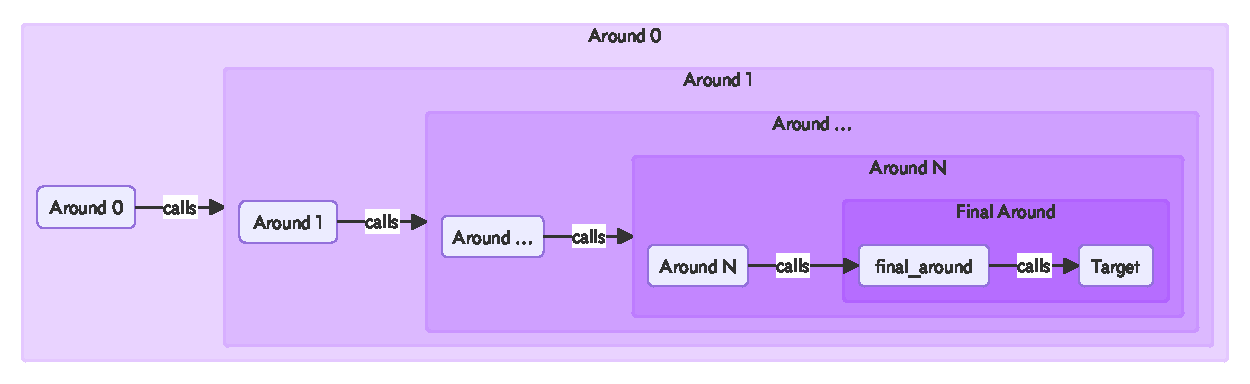
\includegraphics[width=\columnwidth]{40_pydysofu_rewrite/diagrams/nesting_of_around_advice.pdf}
\caption{An informal flowchart showing how around advice nests. Each box shows a
level of nesting of partial functions, and represents the closure of the partial
function constructed at that level of nesting. Nodes in the graph are functions
implementing either the target of advice, \lstinline{final_around}, or a piece
of advice woven against the target.}
\label{fig:levels_of_nesting_arounds}
\end{figure}
% The nested calls this process produces are further illustrated by
% \cref{fig:nested_around_advice_construction_illustration}, which shows how each
% stage of this process nests calls to around advice.
% \begin{figure}
% \centering
% \lstinputlisting[style=footnotesize_pseudocode]{40_pydysofu_rewrite/snippets/around_stages.pseudocode}
% \caption{Pseudocode illustrating the value of the around advice constructed on
% each iteration of the loop illustrated in \cref{fig:final_around_pseudocode}.}
% \label{fig:nested_around_advice_construction_illustration}
% \end{figure}

Line \texttt{57} invokes \lstinline{nested_around}, which in turn invokes every
around advice applied as well as the target. The return value of the target,
possibly modified by around advice, is stored in the variable \lstinline{ret}.


\subsubsection{Encore Advice and Returning from Aspect Hooks}

Encore advice, invoked after a target returns, is implemented on lines
\texttt{60}--\texttt{62} of \cref{fig:build_wrapper_impl}. Any advice
which runs after the target returns is able to inspect and modify the target's
return value if required; line \texttt{62} replaces the copy of the target's
return value with that returned by any advice if the advice returns a
non-\lstinline{None} value.

Line \texttt{63} resets the code object implementing the target using
\lstinline{reset_code_to_previous}, ensuring that any fuzzers that were invoked
had no side-effects lasting after the wrapper function returns. No further work
is required of \pdsfthree{}, and so the wrapper function returns the return value of
the target (or its modified value if changed by any encore advice).


\subsubsection{Error Handling Advice}
\label{error_handling_advice}
The final type of advice supported by \pdsfthree{} is error-handling advice. If a
target raises an exception, it is intercepted by \pdsfthree{}, which will continue to
raise the exception unless error handling advice is applied. 

Line \texttt{66} of \cref{fig:build_wrapper_impl} intercepts a thrown
exception. The underlying code object of the target is reset on line
\texttt{67}, in case it was modified by a fuzzer, to avoid side-effects
remaining after the aspect hooks return. Each error handler applied to the
target is executed on lines \texttt{69}--\texttt{70}. If any ``truthy'' value is
returned by any error handling advice, the exception is not raised and the
caller of the target can continues to execute, oblivious to the exception. A
``truthy'' value is any value which is interpreted as \lstinline{True} in a
boolean expression in Python --- this is any value which is not
\lstinline{None}, \lstinline{0}, or \lstinline{False}.


\subsection{Using \pdsfthree{}}
\label{examples_of_using_pdsf}

An example of an aspect woven into a join-point is shown in
\cref{fig:registering_an_aspect_against_aspecthooks}.

\begin{figure}
    \begin{lstlisting}[style=footnotesize_python]
def prelude_log_invocation(target, *args, **kwargs):
    '''
    Prelude advice to print invocations of a target.
    '''
    print(f"Invoking {target.__name__}")
    
def encore_log_return(target, return_val, *args, **kwargs):
    '''
    Encore advice to print a target's return value
    '''
    print(target.__name__ + " returned value: " + str(return_val))
    
def around_logger(next_around, target, *args, **kwargs):
    '''
    Around advice equivalent to applying both
    prelude_log_invocation and encore_log_return.
    '''
    print("Invoking " + target.__name__)
    return_value = next_around(target, *args, **kwargs)
    print(target.__name__ + " returned value: " + str(return_val))
    return return_value

from pdsf import AspectHooks
with AspectHooks():
    from some_module import some_func

AspectHooks.add_prelude("some_func", prelude_log_invocation)
AspectHooks.add_encore(".*", encore_log_return)
    \end{lstlisting}
    \caption{Complete examples of prelude, encore, and around advice. Prelude
    and encore advice is registered against
    pointcuts described by string-represented regular expressions. The around
    advice is not registered, but is provided to demonstrate the similarities
    between around advice and the combination of prelude and encore advices.}
    \label{fig:registering_an_aspect_against_aspecthooks}
\end{figure}

Lines \texttt{1}--\texttt{11} define functions which can be used as
advice. The first, \lstinline{prelude_log_invocation}, is intended to be run as
prelude advice and so has the function signature
\lstinline{target},~\lstinline{*args},~\lstinline{**kwargs}. It prints the name
of a function before it is invoked. The second, \lstinline{encore_log_return},
is intended to be run as encore advice and so has the function signature
\lstinline{target,}~\lstinline{return_val,}~\lstinline{*args,}~\lstinline{**kwargs}.
It also logs the name of the target function, as well as the value that function
returned.


Lines \texttt{23}--\texttt{25} import a function, \lstinline{some_func}, from a
module \lstinline{some_module} using \lstinline{AspectHooks}. The hooks are
active within the body of the \lstinline{with} block. The function object
imported as
\lstinline{some_func} is the original function wrapped in the aspect hook
implementation shown in \cref{fig:build_wrapper_impl}. Line \texttt{27} applies
prelude advice to the \lstinline{some_func} function by associating
\lstinline{prelude_log_invocation} with the pointcut \lstinline{"some_func"}.
Only functions with the name \lstinline{some_func} will be invoked with this
advice applied. Line \texttt{28} applies the encore aspect
\lstinline{encore_log_return} to the pointcut \lstinline{".*"}, which matches
any function identifier --- as a result, \emph{any} function invocation with
aspect hooks injected will be run with this encore advice applied. As a result,
an invocation of the function \lstinline{some_func} would print its name before
invocation as well as its return value after invocation. 

The around advice defined on lines \texttt{13}--\texttt{21},
\lstinline{around_logger}, is not woven but is shown to demonstrate how prelude
and encore advice can be represented as around advice.

\begin{figure}
    \begin{lstlisting}[style=footnotesize_python]
import ast

def fuzzer_invocation_logger(ast_steps, target, *args, **kwargs):
    '''
    Fuzzer advice which prints the name of the invoked target.
    '''
    print_invoked_func = f"Invoking {target.__name__}"
    print_invocation_ast = ast.parse(print_curr_func)
    return print_invocation_ast.body + ast_steps

from pdsf import AspectHooks
with AspectHooks():
    from some_module import some_func

AspectHooks.add_fuzzer("some_func", fuzzer_invocation_logger)
    \end{lstlisting}
    \caption{Complete example of logging function invocation using a fuzzer instead of the prelude advice shown in \cref{fig:registering_an_aspect_against_aspecthooks}.}
    \label{fig:fuzzer_logging_example}
\end{figure}

\Cref{fig:fuzzer_logging_example} shows a fuzzer which logs function invocations
similar to the example in \cref{fig:registering_an_aspect_against_aspecthooks}.
On line \texttt{7}, a line of Python is stored as a string which prints the name of the
target. This code is parsed into an AST on line \texttt{8}, and the parsed code
is prepended to the target's body on line \texttt{9}. The first thing the target
will do once recompiled by \pdsfthree{} is to execute the line of code shown on line
\texttt{7}, after which the target's implementation is defined as it was
previously. This fuzzer is woven into the target in the same way as in
\cref{fig:registering_an_aspect_against_aspecthooks} in the remainder of the
example.


\subsection{Comparison to Other Weaving Mechanisms}

Import hook weaving is a novel technique for weaving aspect hooks. This section
compares \pdsfthree against other \aop frameworks to determine its novelty and
contribution. As it is not feasible to compare \pdsfthree against \emph{all}
alternative \aop frameworks, it will be compared against
AspectJ~\cite{AspectJLanguageAndTools} and Spring
AOP~\cite{springAOPDocumentation} as these are actively maintained \aop
frameworks which see some industry adoption~\cite{przybylek2018empirical}. As
such, we consider these frameworks representative of the \aop ecosystem at time
of writing. Any claims of novelty made in relation to these frameworks hold in
comparison against other frameworks too; AspectJ and Spring AOP are selected for
illustrative purposes.

% Compare for novelty
\pdsfthree{}'s implementation of \aop weaves aspect hooks into modules which may
contain join points. This allows join-points to be determined at runtime. Advice
is implemented in the form of Python functions. Weaving is performed when
modules are imported. Only a module which imports join-points with
\lstinline{AspectHooks} will observe aspect hooks woven into those join-points;
other modules within the same program which do not import with
\lstinline{AspectHooks} will observe no \aspectoriented behaviour when invoking
those join-points. This is described in detail in
\cref{local_aspect_hook_effects}. In that section
\cref{fig:isolated_aspect_hook_weaving_illustration} is shown, which contains a Python program
made of several modules which illustrates this. Weaving is dynamically performed
at runtime, and can happen whenever a package is imported. As Python supports
re-importing packages, \pdsfthree can weave aspect hooks even when a package is
already loaded. This allows \pdsfthree users to determine whether they require
aspect hooks to be woven at any point in program execution. Also, \pdsfthree{}'s
application of aspect hooks --- and weaving of aspects --- appears only in the
parts of a program it effects. As \pdsfthree weaves aspect hooks when packages
are imported and Python packages are conventionally imported at the top of a
file, \pdsfthree users can easily clarify whether any \aspectoriented behaviour
is expected in their program, and where that behaviour occurs.

AspectJ offers multiple mechanisms for weaving aspect hooks: compile-time
weaving is offered through rewriting binary \lstinline{.class}
files~\cite{aspectj-bytecode-weaving-documentation} and runtime
weaving\footnote{AspectJ refers to runtime weaving as ``load-time weaving'',
because its implementation specifically weaves hooks when classes are loaded.}
is offered through modified classloaders~\cite{aspectj_ltw_docs}. Neither
mechanism supports weaving aspect hooks into already-loaded classes. The
application of aspects is controlled via \lstinline{.xml} configuration files in
both cases. Aspects woven into a class are observed by all users of that class.
Aspects are written in Java, using a superset of the Java language\footnote{The
superset of the Java language used to implement aspects is called AspectJ.}, so
an extension to Java is required in order to use it. As AspectJ join-points are
specified in configuration files, users of AspectJ must check any configuration
files for their program to understand whether any part of their program will
exhibit \aspectoriented behaviour. The negative impact on program legibility
this causes is often cited as a limitation of
\aop{}~\cite{Constantinides04aopconsidered,steimann06paradoxical,przybylek2010wrong,przybylek2018empirical}.

Spring AOP is designed with AspectJ compatibility in
mind~\cite{introducing_spring_aop_chapter_integration_with_aspectj}, and so
supports the AspectJ superset of the Java language and AspectJ's
\lstinline{.xml} configuration format. However, Spring AOP also offers its own
aspect hook weaving technique: proxy objects which act as adapters between
join-points and other parts of a program that invoke them. Proxy objects act as
proxies of join-points. This allows fine-grained weaving of aspect hooks, as a
program only needs to construct proxy objects for any join-points in use to
support \aop{}. It also allows for flexible weaving of aspect hooks, as the
construction of a proxy object can occur at any point in a program's execution.
However, this weaving mechanism complicates code comprehension: any part of a
program using a non-proxied reference to a join-point will see no
\aspectoriented behaviour. For example, this occurs when the proxied object
invokes methods on itself, as an object's \lstinline{this} reference is not
proxied through Java's proxy API. Overcoming this limitation requires a
join-point to implement additional logic to call its own methods through a proxy
if it exists, which breaks \aop{}'s philosophy of
obliviousness~\cite{filman2000aspect}. Spring AOP supports using AspectJ to
weave aspect hooks and apply aspects instead of or in addition to its own aspect
weaving, which may complicate program comprehension by adding additional
complexity to determining whether any part of a program exhibits \aspectoriented
behaviour. This is because both weaving techniques must be checked to form a complete
understanding of program behaviour. 

Import hook weaving offers improved code comprehension compared to other weaving
mechanisms, because it offers simple semantics around \aspectoriented behaviour:
modules which import other modules with \lstinline{AspectHooks} observe
\aspectoriented behaviour, and any other modules do not. Confirming whether a
program exhibits \aspectoriented behaviour for conventionally written Python
programs is as simple as checking the top of a file for references to
\lstinline{AspectHooks}. This compares favourably to other techniques, which
rely on program configuration to identify join-points and complicate the
invocation of \aspectoriented program behaviours with wrapper mechanisms such as
proxy objects. Import hook weaving therefore improves on existing aspect hook
weaving mechanisms by offering a novel solution to the problem of
\aspectoriented programs' legibility.



% \begin{multilisting}
%     \sublstinputlisting[1]{40_pydysofu_rewrite/snippets/isolated_hook_weaving/main.py}{main.py}
%     \sublstinputlisting[1]{40_pydysofu_rewrite/snippets/isolated_hook_weaving/moduleA.py}{moduleA.py}
%     \sublstinputlisting[1]{40_pydysofu_rewrite/snippets/isolated_hook_weaving/moduleB.py}{moduleB.py}
%     \sublstinputlisting[1]{40_pydysofu_rewrite/snippets/isolated_hook_weaving/joinpointModule.py}{joinpointModule.py}
%     \sublstinputlisting[1]{40_pydysofu_rewrite/snippets/isolated_hook_weaving/aspects.py}{aspects.py}
% \begin{figure}
%     \caption{Example Python project with multiple modules, which demonstrate how \pdsfthree isolates \aspectoriented behaviour to affect only modules which import join-points with \lstinline{AspectHooks}.}
% \label{fig:isolated_aspect_hook_weaving_illustration}
% \end{figure}
% \end{multilisting}
% \end{figure}


% Summarise contribution briefly.



\subsection{Strengths and Weaknesses of Import Hooks}\label{subsec:pdsf3importhooklimitations}

As a technique for weaving aspect hooks, this new method provides multiple
benefits.

\correctionnote{\emph{CONTRIBUTIONS OF IMPORT HOOK WEAVING MUST BE GIVEN, AND
COMPARISONS TO OTHER AOP FRAMEWORKS MUST BE MADE}}

\correctionnote{
    This could be co-opted to be a discussion of import hook weaving's
    contributions. Maybe another subsec comparing import hook weaving to
    AspectJ? PROSE?
}

\Needspace{3\baselineskip}
\begin{description}
    \item[Local Aspect Weaving.] Application of aspect hooks is straightforward
        from the perspective of a modeller using \pdsfthree{}, whose code clearly
        applies aspect hooks and does so in a legible way for future
        maintainers. This is guaranteed by \pdsfthree{}'s weaving of aspect hooks
        only in the scope of the program where they are applied: hooks are woven
        into the module where it is imported using \lstinline{AspectHooks}, but
        not in other parts of the program. Import hooks' explicit application of
        hooks to modules makes clear the specific areas of a program where
        advice could be applied.

    \item[Legible Obliviousness.] While join points are oblivious to potential
        aspect application, callers of join points are responsible for weaving
        the advice they want to apply. This leaves signs of \aspectorientation{}
        in helpful places within a codebase for its maintainers. Aspect hooks
        can be injected into specific functions imported from a module or the
        entire module depending on the way modules are imported, allowing for
        total weaving or actual hook weaving depending on their preferences.
        This is because, in Python, \lstinline{import X} will import a module
        named \lstinline{X}. However, the syntax \lstinline{from X import A, B, C} imports only
        the symbols \lstinline{A}, \lstinline{B}, and \lstinline{C} from the
        module \lstinline{X}. Using this, aspect hooks can be injected into
        subsets of a module, rather than the entire module.
        
        As well as allowing greater flexibility for the convenience of a
        developer, the performance of import hooks is improved in comparison to
        replacing the \lstinline{__getattribute__} method on a class. In
        comparison to \pydysofu{}, which used the
        latter technique, the new implementation's import hooks are weave-able
        at a more granular level. This is because import hooks introduce
        additional program logic to procedures such as functions and methods,
        rather than all attributes of a class as did
        \pydysofu{}'s old mechanism. Less overhead is expected as a result.\revnote{I should really
        have numbers for this.}

    \item[Requires No Special Accommodations.] As with \pydysofu{},
        \pdsfthree{}'s import hooks are implemented entirely in Python and
        require no special support from language runtime modifications. Other
        aspect orientation frameworks often require special languages for
        describing aspects, such as AspectJ~\cite{AspectJLanguageAndTools}, or
        runtime plugins, such as PROSE~\cite{popovici2002PROSE}. \pdsfthree{}'s
        import hooks are written entirely in native Python, and can be used in
        existing software projects without requiring any special accommodations.
        Minimising the difficulty of adopting \pdsfthree{} is a desirable property of
        its design: if it can be used without modifying existing codebases,
        researchers' pre-existing models \& simulations can adopt \pdsfthree{} with
        minimal engineering effort.
\end{description}

There are also caveats to this approach. As aspect hooks are woven in
\pdsfthree{} via Python's import functionality, any procedure which is not
imported from a module cannot have aspect hooks attached. \revnote{Consider
adding local namespace weaving to pdsf3: should be easy to implement as a cheeky
little monkey-patch\ldots{}} However, as aspect orientation is primarily
concerned with a separation-of-concerns approach to software architecture,
targets are expected to be scattered across many modules, so this does not
appear to be a significant limitation. The notion that targets reside in other
modules than those where weaving takes place holds in other \aspectoriented{}
simulation \& modelling codebases: for example, those from
\citet{wallis2018caise} as described in \cref{chap:prior_work}.



\section{Optimisations}
\label{pdsf3_optimisations}

Additional features were implemented in \pdsfthree to make it more useful for
research software engineering, and to optimise performance where necessary. The
optimisations introduced are deep hook weaving, non-dynamic weaving, priority
ordering of aspect application and cached fuzzing. They are explained
individually in the following subsections.

\subsection{Deep Hook Weaving}\label{deep_hook_weaving}

Ordinarily \pdsfthree weaves aspect hooks into an imported module, but not modules
imported by that module. This is to avoid overheads incurred by patching
commonly-used libraries with aspect hooks in scenarios where they are not
intended to be join-points. However, this behaviour may be desirable at times.
Deep hook weaving enables weaving of aspect hooks into all potential join-points
by not only applying hooks to functions and methods which were imported by the
original module, but also to any modules which the original module imports. The
feature is enabled by toggling a flag set on the \lstinline{AspectHooks} class,
as shown in \cref{fig:enabling_deep_apply}.

\begin{figure}[h]
    \begin{lstlisting}[style=footnotesize_python]
from pdsf import AspectHooks
AspectHooks.deep_apply = True
    \end{lstlisting}
    \caption{Code snippet enabling deep hook weaving}
    \label{fig:enabling_deep_apply}
\end{figure}

Deep hook weaving introduces performance overhead due to additional checks for
aspects which were woven dynamically. However, it is possible that the modules
which contain desired join points are not imported directly by a developer, but
are available to them indirectly through another package they make use of. It is
also possible that a developer may look to instrument the entirety of a call
stack without attaching a debugger to a process, for example to examine call
stacks, to perform security checks, for fuzz testing, or for custom logging
within third-party and built-in modules. These use-cases require aspect hooks to
be woven more deeply than to only one module. In these examples, \pdsfthree{}'s
default behaviour is insufficient. Deep weaving is provided to support these use
cases.

\begin{figure}
    \begin{lstlisting}[style=footnotesize_python]
from_mod = getattr(item, "__module__", None) == mod.__name__
if from_mod or AspectHooks.deep_apply:
    if isfunction(item) or ismethod(item):
        setattr(target_object, item_name, build_wrapper(item))
    elif isclass(item):
        apply_hooks(item)
    \end{lstlisting}
    \caption{The implementation of \pdsfthree{}'s ``deep weaving'' option, which
    allows aspect hooks to be injected into recursive imports or only into the
    first module being imported, reducing overhead if a specific join-point of
    advice is targeted by a developer. Edited slightly for readability.}
    \label{fig:deep_weaving_optimisation_implementation}
\end{figure}

The implementation of deep weaving is shown in
\cref{fig:deep_weaving_optimisation_implementation}, a snippet of the
\lstinline{apply_hooks} function which monkey-patches module objects during
import to inject aspect hooks. The feature is implemented as an \lstinline{if}
statement which ensures that the condition checking whether a module or class
object originated from the original import always evaluates to \lstinline{True}, as seen
on line \texttt{2} in the figure. This check can effectively be disabled by
ensuring the condition always evaluates to \lstinline{True}, meaning that all
imported modules and classes would be woven into, even if they did not belong to
the first module object imported.

\pdsfthree requires an option for deep hook weaving because it weaves aspect
hooks when modules containing possible join-points are imported rather than when
pointcuts are specified. Similar functionality is offered by \aop frameworks
such as AspectJ and PROSE, but concepts in other frameworks differ by virtue of
their different weaving mechanisms. For example, AspectJ weaves aspect hooks
into every Java class by default but can configure this to be more specific
through the configuration of its weaver~\cite{}. An example AspectJ
configuration which weaves aspect hooks selectively and controls the recursive
weaving of hooks shown in \cref{fig:aspectj_configuration_for_hook_nesting}.
AspectJ disallows the weaving of advice into delegated classloaders when weaving
advice at runtime~\cite{aspectj_ltw_docs}, which prevents classes repeatedly
weaving advice into others they import or load (which is the use case for
AspectJ most analogous to Python modules importing other Python modules). PROSE
weaves aspects as join-points are called using a just-in-time (JIT)
compiler~\cite{dynamicAOPWithProse}. Callbacks are woven into join-points when
aspects are applied, alleviating the need to weave aspect hooks into classes and
so avoiding the need for deep hook weaving by design. Deep hook weaving is
therefore a novel solution to the recursive weaving of modules, but is not a
\emph{unique} solution to that problem.

\begin{figure}
\begin{lstlisting}[style=footnotesize_xml]
<aspectj>
    <weaver>
        <!-- Weave hooks within the foo.bar or com.example namespaces -->
        <include within="foo.bar.*"/>
        <include within="com.example.*"/>

        <!-- Do not weave types within the "bar" namespace -->
        <exclude within="bar.*"/>
    </weaver>
</aspectj>
\end{lstlisting}
\caption{An example aspectj configuration which weaves aspect hooks rec}
\label{fig:aspectj_configuration_for_hook_nesting}
\end{figure}


\subsection{Static Weaving}
\label{static_weaving}

\pdsfthree{}'s runtime weaving of aspects allows them to be applied dynamically.
However, programs may be written which apply aspects at join-points which do not
dynamically change. For example, an aspect may implement a program modification
to affect one specific join-point, which is written as an aspect to support the
simple inclusion or exclusion of the feature the aspect implements. In this
scenario and others like it, the join-points used by aspects would never change.
As a result, the dynamic weaving of \pdsfthree introduces unnecessary runtime
overhead: aspects will never be \emph{unwoven}, but \pdsfthree{}'s dynamic
behaviour continually searches for aspects applied to a join-point on every
invocation to ensure any unwoven advice is not invoked. Repeated searches for
advice are unnecessary if join-points do not change.

\begin{figure}[h]
    \begin{lstlisting}[style=footnotesize_python]
from pdsf import AspectHooks
AspectHooks.treat_rules_as_dynamic = True
    \end{lstlisting}
    \caption{Code snippet enabling dynamic weaving}
    \label{fig:enabling_dynamic_weaving}
\end{figure}

To avoid this overhead in scenarios where it is not required, an optimisation
can be introduced where aspects are woven statically. \pdsfthree can cache the
aspects applied when any callable wrapped by an aspect hook is invoked for the
first time. On its first execution in this mode, the aspect hook stores the set
of aspects it matched to the invoked target, and future invocations retrieve the
set of aspects to apply from the cache. This avoids expensive regular expression
matches,
\revnote{
    The use of regexes for matching aspects to join points isn't explained at
    time of writing.
}
which fail in all cases but those where an invoked target is to be augmented by
the application of an individual aspect the regular expression is paired
with.
\revnote{
Add metrics here on the performance implications if there's time; they're pretty
significant, I actually added them because the regex matches slowed my own code
down to a crawl. Our experiments make use of static weaving for this reason.
}

For performance reasons, the default behaviour of \pdsfthree is to use static
weaving. Dynamic weaving is enabled by toggling the
\lstinline{treat_rules_as_dynamic} flag on the \lstinline{AspectHook} class, as
similarly to enabling or disabling deep hook weaving (see
\cref{deep_hook_weaving}). A code snippet demonstrating this is shown in
\cref{fig:enabling_dynamic_weaving}.

Static weaving is similar to the ability to turn on or off dynamic behaviour in
other \aop frameworks which offer dynamic aspect weaving. Static weaving
therefore brings \pdsfthree closer to feature parity with other \aop frameworks.
An example of an analogous feature in other frameworks is AspectJ's compile-time
loading of aspects by injecting advice into join-points by rewriting the
\lstinline{.class} files corresponding to each
join-point~\cite{aspectj-bytecode-weaving-documentation}. 

\subsection{Priority Ordering of Aspect Application}
\label{aspect_priority_support}

As dynamic weaving allows for the conditional application of aspects, it may be
that the order in which aspects are woven is not the order in which they are
intended to be \emph{invoked}: different aspects may have different priorities.
To support these use cases, aspects can be applied with a priority, which is
used to sort them when aspects are dynamically searched for and invoked on
target invocation. This feature is disabled by default, but can be enabled using
the code snippet shown in \cref{fig:enabling_priority_sorting_of_aspects}.

\begin{figure}[h]
    \begin{lstlisting}[style=footnotesize_python]
from pdsf import AspectHooks
AspectHooks.manage_ordering = True
    \end{lstlisting}
    \caption{Code snippet enabling priority ordering of aspect application in \pdsfthree{}.}
    \label{fig:enabling_priority_sorting_of_aspects}
\end{figure}

As mentioned in \cref{urgency_mentioned_in_passing}, when aspects are registered
against the \lstinline{AspectHooks} class an optional \lstinline{urgency}
parameter is available. This parameter is an integer representation of the
aspect's ``priority'' with the same semantics as in a priority queue. Higher
numbers represent more urgent application, so high-urgency aspects are applied
before low-urgency aspects. Aspects with no urgency applied default to
\lstinline{urgency=0}.

Other \aop frameworks also offer priority ordering of aspect application,
although the feature is relatively novel in the
community~\cite{jalali2012aspect}. For example, AspectJ allows aspects to be
declared with a precedence ordering which explicitly notes which aspects should
run in which order for a given
join-point~\cite{aspectj-advice-precedence-documentation}. An example AspectJ
configuration which specifies precedence of advice application is given in
\cref{fig:aspectj-advice-precedence-config-example}.

\begin{figure}
\centering
\begin{lstlisting}[style=footnotesize_xml]
<aspectj>
    <aspects>
        <concrete-aspect name="com.thesis.ExampleAdviceClass"
                         precedence="logInvocation, checkSecurityProperties, *"/>
    </aspects>
</aspectj>
\end{lstlisting}
\caption{An example AspectJ configuration which specifies precedence of advice
application~\cite{aspectj-advice-precedence-documentation}.}
\label{fig:aspectj-advice-precedence-config-example}
\end{figure}


\subsection{Cached Fuzzing}
\label{subsec:cached_fuzzing}

Invoking fuzzers requires parsing Python ASTs and compiling Python code objects,
which introduces overhead in their implementation. However, some use-cases for
fuzzers will produce the same AST every time they fuzz their target. Examples
include the function invocation logger given as an example in
\cref{fig:fuzzer_logging_example} and the advice written to implement
experiments in \cref{chap:experiment_setup} such as
\cref{fig:prior_distribution_implementation}, both of which inject the same AST
step nodes at the same point in their target on every invocation. To alleviate
this overhead, the compiled result of applying fuzzers to an aspect can be
cached. This is enabled using the \lstinline{cache_fuzz_results} attribute of
the \lstinline{AspectHooks} class can be set, as shown in
\cref{fig:enabling_fuzzer_caching}.

\begin{figure}[h]
    \begin{lstlisting}[style=footnotesize_python]
from pdsf import AspectHooks
AspectHooks.cache_fuzz_results = True
    \end{lstlisting}
    \caption{Code snippet enabling priority ordering of aspect application}
    \label{fig:enabling_fuzzer_caching}
\end{figure}


\begin{figure}
    \begin{lstlisting}[style=footnotesize_python]
if fuzzers is not None and fuzzers != []:
    cache_key = tuple([str(fuzzer) for fuzzer in fuzzers] + [str(target)])

    if self.cache_fuzz_results and self._cached_fuzzer_applications.get(cache_key) is not None:
        compiled_fuzzed_target = self._cached_fuzzer_applications[cache_key]
    else:
        code = dedent(inspect.getsource(t))
        target_ast = ast.parse(code)
        funcbody_steps = target_ast.body[0].body

        for fuzzer in fuzzers:
            non_inline_changed_steps = fuzzer(funcbody_steps, *args, **kwargs)
            if non_inline_changed_steps:
                funcbody_steps = non_inline_changed_steps

        target_ast.body[0].body = funcbody_steps
        compiled_fuzzed_target = compile(target_ast, "<ast>", "exec")
        if self.cache_fuzz_results:
            self._cached_fuzzer_applications[cache_key]=compiled_fuzzed_target

    if not isinstance(t, FunctionType):
        t.__func__.__code__ =  compiled_fuzzed_target.co_consts[0]
    else:
        t.__code__ = compiled_fuzzed_target.co_consts[0]
    \end{lstlisting}
    \caption{Implementation of aspect hooks for fuzzers, which includes the
    optimisation for cached fuzzing. Fuzzed targets are cached on line
    \texttt{19}, and used on line \texttt{5} instead of re-running fuzzing
    advice if cached fuzzers are enabled by setting the
    \lstinline{cache_fuzz_results} attribute of the \lstinline{AspectHooks}
    class.}
    \label{fig:implementation_fuzzer_cache_pdsf}
\end{figure}

Caching fuzzer output allows \pdsfthree{} to compile the output of any applied fuzzer
on their first invocation. Its implementation is shown in
\cref{fig:implementation_fuzzer_cache_pdsf}. On line \texttt{2}, a unique key
for the advice applied to an invoked target is constructed. This key changes if
dynamic fuzzing is enabled (see \cref{static_weaving}), so a cache miss occurs
if fuzzing aspects are added or removed between target invocations. Lines
\texttt{4}--\texttt{5} circumvent the implementation of fuzzer aspect hooks and
retrieve a cached fuzzed target instead if the key constructed on line
\texttt{2} exists in the cache of fuzzed targets. If it does not, fuzzing
continues as normal, and the output of running any applied fuzzers is added to
the cache on line \texttt{19} to be used when the target is next invoked.

As fuzzers are a unique feature of \pydysofu and \pdsfthree{}, cached fuzzing
does not exist in other \aop frameworks. It is an improvement over \pydysofu and
thus a novel contribution in the design of \aop frameworks.


\section{Summary}
\label{pdsf3_discussion}

\pdsfthree{} improves over both existing \aop{} frameworks and its own previous
incarnation, \pydysofu{}. It introduces a new technique of weaving aspect hooks
when importing modules, improving its design over a typical \aspectorientation{}
framework by making use of Python's \lstinline{with} keyword when weaving hooks.
This improves the legibility of \aspectoriented{} programs through more explicit
application of aspect hooks. In addition, many optimisations are introduced
\pydysofu did not offer: aspect hooks can be injected only into a module being
imported, or recursively into every module imported in the process of importing
the first one; aspects can be woven dynamically or statically, reducing
overheads when developers do not require dynamic behaviour; and the order of
application of aspects can be made explicit by developers when this
functionality is required.

\pdsfthree{} also provides opportunities for improvements and
for future work. Our intended use case for aspect orientation for simulation \&
modelling is in scientific codebases specifically: direct integration with the
scientific package ecosystem (which is vibrant in Python's community) should be
made. A good initial project would be integration of aspect application in
sciunit tests~\cite{sciunit_primer}, which represent experiments on a model as
unit tests. The potential to encode hypotheses as advice (discussed in
\cref{sciunits_for_unrealistic_states}) or as alternative behaviours within a
model (described in \cref{chap:experiment_setup} and evaluated in
\cref{chap:experimental_results}) has lots in common with SciUnit's design goal
of formalising hypotheses as unit tests. As both projects are written in Python
and have similar use-cases, there is seemingly some potential for integration
between these projects and collaboration with the SciUnit team. A discussion on
potential use cases of \pdsfthree together with existing research software
engineering technologies is provided in \cref{sciunits_for_unrealistic_states}.

\Cref{chap:experiment_setup} and \cref{chap:experimental_results} use \pdsfthree
to design experiments which investigate \aspectoriented{} simulations \& models,
and evaluate their results.

\subsection{Contributions}
\label{pdsf3_contributions_summarised}

\pdsfthree contributes import hook weaving to \aop{} framework design. This
novel type of weaver introduces aspect hooks to join-points without making
changes to a language runtime or weaving aspect hooks directly into a program
before or after compilation. 

Import hooks address common criticisms of the \aspectoriented{} paradigm by
improving the legibility of an \aop{} program. This is achieved by limiting the
scope of a program which aspect hooks are woven into. This has the effect of
reducing the number of points in a program that \emph{could} weave aspect hooks
into a join-point, so developers who need to understand a program only need to
follow a function's call stack to observe whether that function could have
aspects applied to it. This is because \pdsfthree{}'s aspect hooks are woven in
predictable parts of a program that are easily reviewed: import statements,
which are written at the top of a Python program by convention.
\correctionnote{
  Maybe say more about the impact of import hook weaving here --- I need to
  justify its novelty and discuss its contributions in more detail anyway, so
  revisit after that's written. 
}


% - import hook weaving
%   - legibility improved because…:
%     - use of AOP is made obvious in codebase by…
%     - signposting to users by taking advantage of Python's convention to import
%   at top of file
%   - import hooks only exist where a package is imported — other uses of a
%   package are not affected
%   - this makes it easy to determine whether a given use of a package is affected
%   by AOP: look through the call stack in the worst case, top of current file in
%   best case.
%   - pydysofu is also improved on by addressing its shortcomings:
%     - improvements targeting efficiency
%     - implementation of missing features i.e. error handling aspects
%     - python3 support
%   - I'm sure there's loads of other things to write here too
%   - Remember that there _must_ be a comparison here against other AOP frameworks.


\pdsfthree also contributes new optimisations to \aop{} framework design: cached
fuzzers. These concern fuzzing aspects, introduced by \pydysofu, which make
changes to their target when invoked. \pydysofu was previously the only \aop{}
framework which offered these join-points, but its implementation of fuzzing
aspects caused targets to be recompiled on every invocation, regardless of
whether the fuzzer's output was the same on every invocation. To avoid this
overhead, \pdsfthree offers a new type of optimisation which caches the output
of fuzzing advice on its first invocation and re-uses its output on future
invocations. This is a novel optimisation for \aop{} frameworks, as no other
framework implementing fuzzing aspects offers it to date.

Finally, \pdsfthree{} improves on \pydysofu{}'s design to make the framework more
appropriate for use in research software engineering practice. This is achieved
through the introduction of new join-points such as exception handlers and the
ability to specify the ordering of aspect application. \pdsfthree also changes
the underlying mechanisms used to weave aspect hooks to make the framework
compatible with versions of Python which are still maintained.



